\begin{frame}
  \frametitle{Danger of Pointers}
  \begin{itemize}
    \item Pointers can refer to arbitrary memory
    \item Reading/writing these pointers is dangerous
          \begin{itemize}
            \item Can overwrite other variables/objects
          \end{itemize}
    \item Can lead to randomly occurring crashes
  \end{itemize}
\end{frame}

\begin{frame}
  \frametitle{Example}
  \code[frame=lines,language=c++14]{example4.cpp}
  \begin{itemize}
    \item Initializer pointer with 5
    \item \texttt{*p = 1} writes one to memory location with address 5
    \item Just don't do it
  \end{itemize}
\end{frame}

\begin{frame}
  \frametitle{Dangling Pointers}
  \begin{columns}
    \column{6cm}
    \code[frame=lines,language=c++14,font=\small]{dangling.cpp}
    \column{4cm}
    \begin{center}
      \begin{tikzpicture}[scale=.5,transform shape,
                          stack frame/.style={anchor=north west,minimum width=4cm,minimum height=1cm,fill=red,opacity=.75,text opacity=1}]
        \draw (0,0) grid ++(4,-4);

        \node[stack frame] at (0,0) {q};

        \visible<3-6>{
          \node[stack frame] at (0,-1) {
            \only<3>{x}%
            \only<4->{x = 2}
          };
          \node[stack frame] at (0,-2) {p};
        }

        \only<5-6>{
          \draw[-latex] (4,-2.5) -- ++(1,0) -- ++(0,0.9) -- ++(-1,0);
        }

        \only<6->{
          \draw[-latex] (4,-0.5) -- ++(1,0) -- ++(0,-0.9) -- ++(-1,0);
        }

      \end{tikzpicture}
    \end{center}
  \end{columns}
  \begin{overprint}
    \onslide<1>
    \begin{center}
      \texttt{q} is allocated on the stack
    \end{center}
    \codeunderlinex{dangling q}

    \onslide<2>
    \begin{center}
      \texttt{foo} is called
    \end{center}
    \codeunderlinex{dangling call}

    \onslide<3>
    \begin{center}
      \texttt{x} and \texttt{p} are allocated on the stack
    \end{center}

    \onslide<4>
    \begin{center}
      \texttt{x} is initialized
    \end{center}
    \codeunderlinex{dangling x}

    \onslide<5>
    \begin{center}
      \texttt{p} is initialized to point to \texttt{x}
    \end{center}
    \codeunderlinex{dangling p}

    \onslide<6>
    \begin{center}
      \texttt{q} receives the result of calling \texttt{foo} \\
      It too points to \texttt{x}
    \end{center}

    \onslide<7>
    \begin{center}
      \texttt{foo}'s stack frame is popped off the stack
    \end{center}

    \onslide<8>
    \begin{center}
      \texttt{q} points to freed memory \\
      It is now a \emph{dangling pointer}
    \end{center}
  \end{overprint}
\end{frame}

\begin{frame}
  \frametitle{Dangling Pointers}
  \begin{itemize}
    \item Using a dangling pointer leads to undefined behaviour
          \begin{itemize}
            \item Program might still seem to function properly for a while
            \item Can lead to randomly occurring bugs later on
          \end{itemize}
    \item Multiple ways of ending up with dangling pointers
    \item Returning a pointer to a local is one such way
    \item Therefore important to know what gets deallocated when
    \item This kind of manual memory management is a major source of bugs
  \end{itemize}
\end{frame}


%%% Local Variables:
%%% mode: latex
%%% TeX-master: "pointers"
%%% End:
